\chapter{Initial Implementation}
\label{ch:impl}

\section{Code structure}
All the code is in one repository on GitHub, \texttt{alikhairyy/trustlance-poc}. The \texttt{contracts/} and \texttt{risk-engine/} folders come from Milestone~1. The \texttt{server/} and \texttt{web/} folders are new in this milestone.

\begin{lstlisting}
trustlance-poc/
|-- contracts/       MilestoneEscrow.sol (escrow, roles, 7-day hold, appeal, pause)
|-- server/
|   |-- index.js     starts the app on a local chain and adds demo accounts
|   |-- app.js       builds the Express app from its services
|   |-- db/          schema.sql (8 tables), index.js (SQLite through sql.js)
|   |-- middleware/  auth.js (JWT login and role checks)
|   |-- routes/      auth.js, jobs.js, milestones.js, arbiter.js
|   `-- services/    chain.js, risk.js, walletFeatures.js, notifications.js
|-- web/             index.html, app.js, styles.css (the three dashboards)
|-- risk-engine/     engine.py, wallet_model.py, audit_log.py, predict_cli.py
|-- test/            contract tests and api/api.test.js
`-- docs/            SRS.md, diagrams/, SECURITY.md, DATASET.md, BENCHMARK.md
\end{lstlisting}

\section{What is implemented}
The brief asks for at least 25\% of the final system, for example backend modules, a database schema or UI screens. All three exist:

\begin{itemize}
\item \textbf{Backend modules.} REST API with registration and login, jobs, proposals, milestones and the arbiter's queue. Every route checks the user's role and whether the user belongs to the job.
\item \textbf{Database schema.} Eight tables, created when the server starts (Figure~\ref{fig:er}).
\item \textbf{UI screens.} A login page, a dashboard for each role, a job page with milestones, and a profile page (Figures~\ref{fig:ui-client} and~\ref{fig:ui-arbiter}).
\end{itemize}

The new code is connected to the Milestone~1 work. Accepting a proposal deploys a real escrow contract on the local chain. Submitting work runs the real Python model, and a high score makes the contract itself refuse the client's approval.

Two features are stubs with their gaps named in the code: notifications are stored in the database but not delivered, and the ratings route answers \texttt{501 Not Implemented}. Counting the 20 functional requirements, 13 are done, 2 are partial, 2 are stubs and 3 are planned.

\begin{figure}[htbp]
\centering
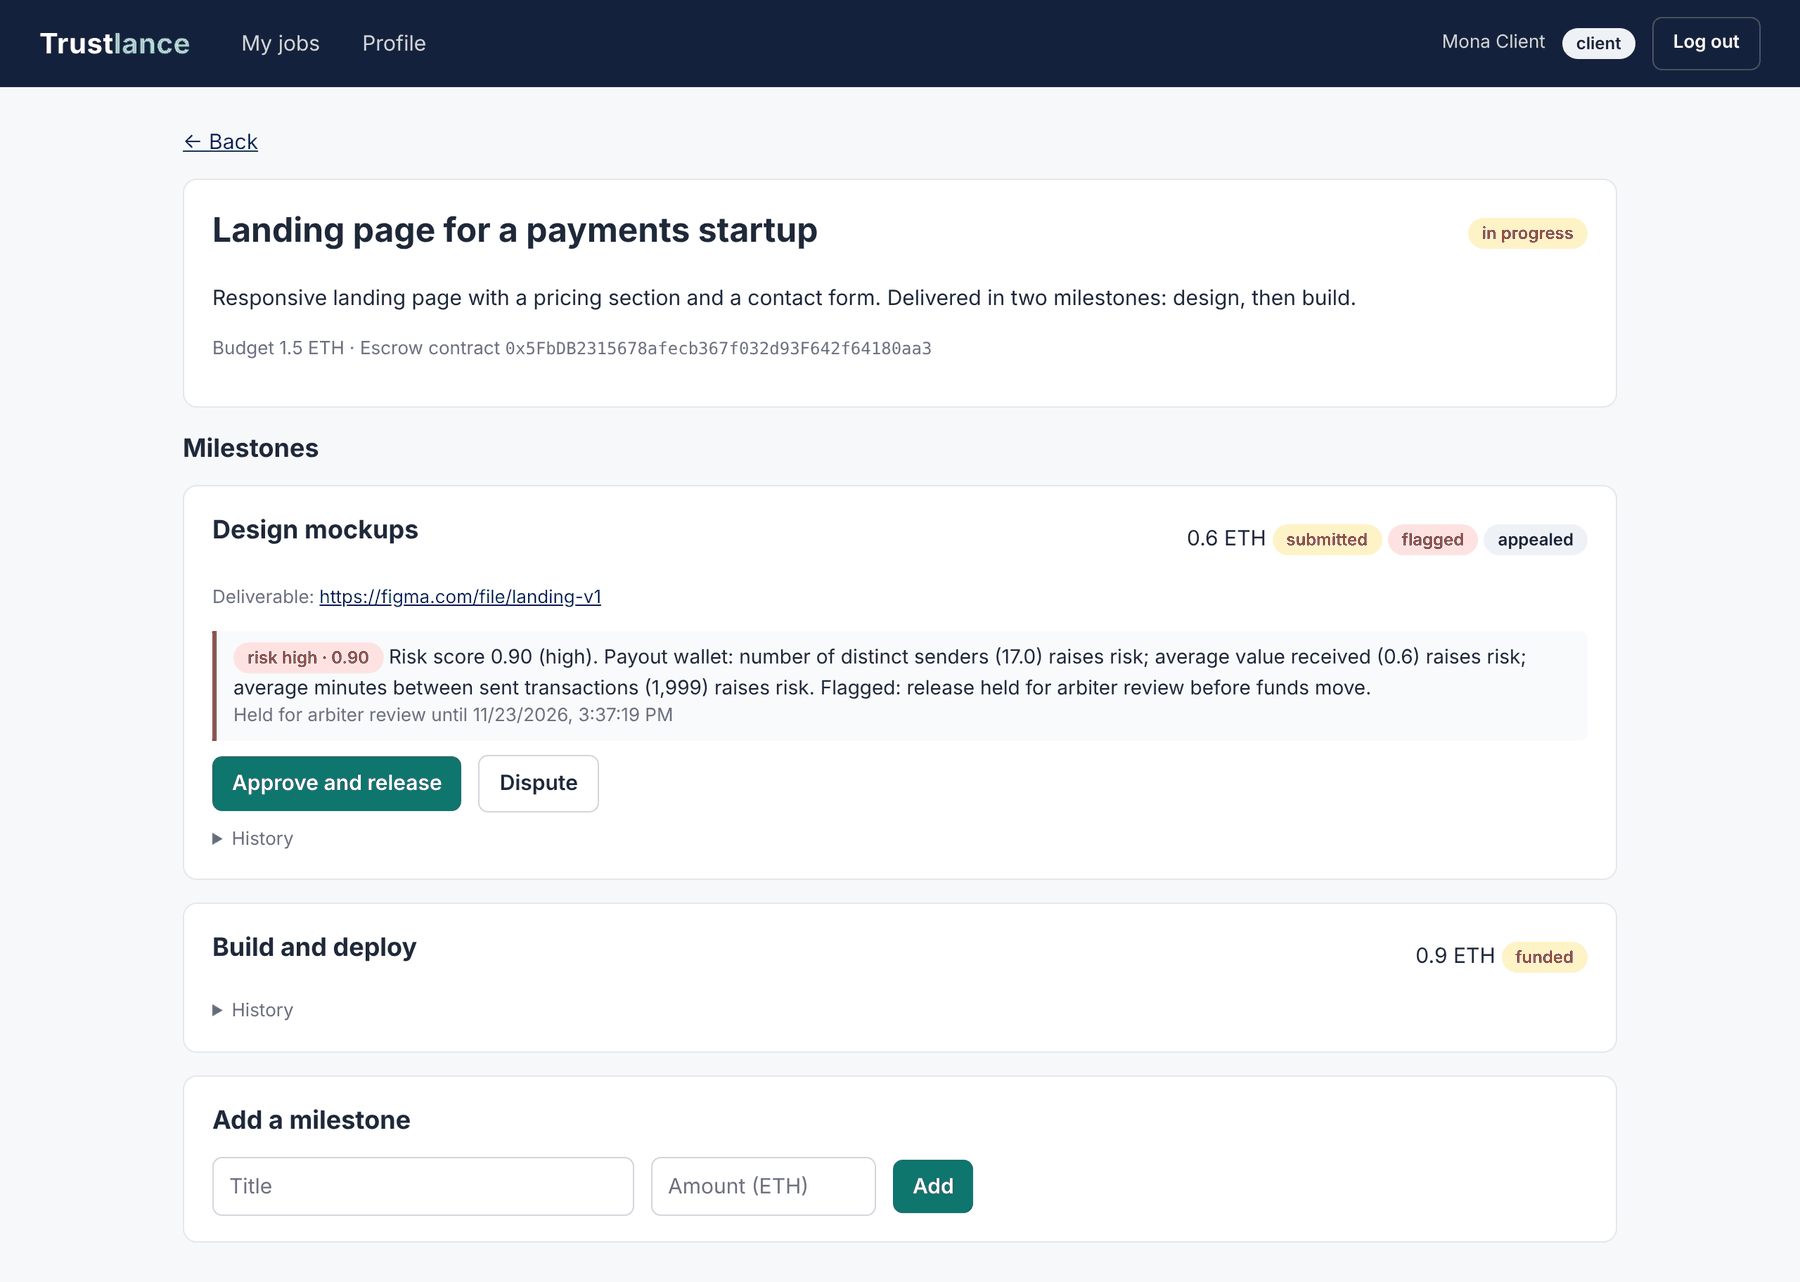
\includegraphics[width=0.92\textwidth]{figures/ui_job_client.png}
\caption{Client's job page. The first milestone was submitted by a freelancer whose payout wallet scored 0.90, so it is flagged, held for seven days and appealed.}
\label{fig:ui-client}
\end{figure}

\begin{figure}[htbp]
\centering
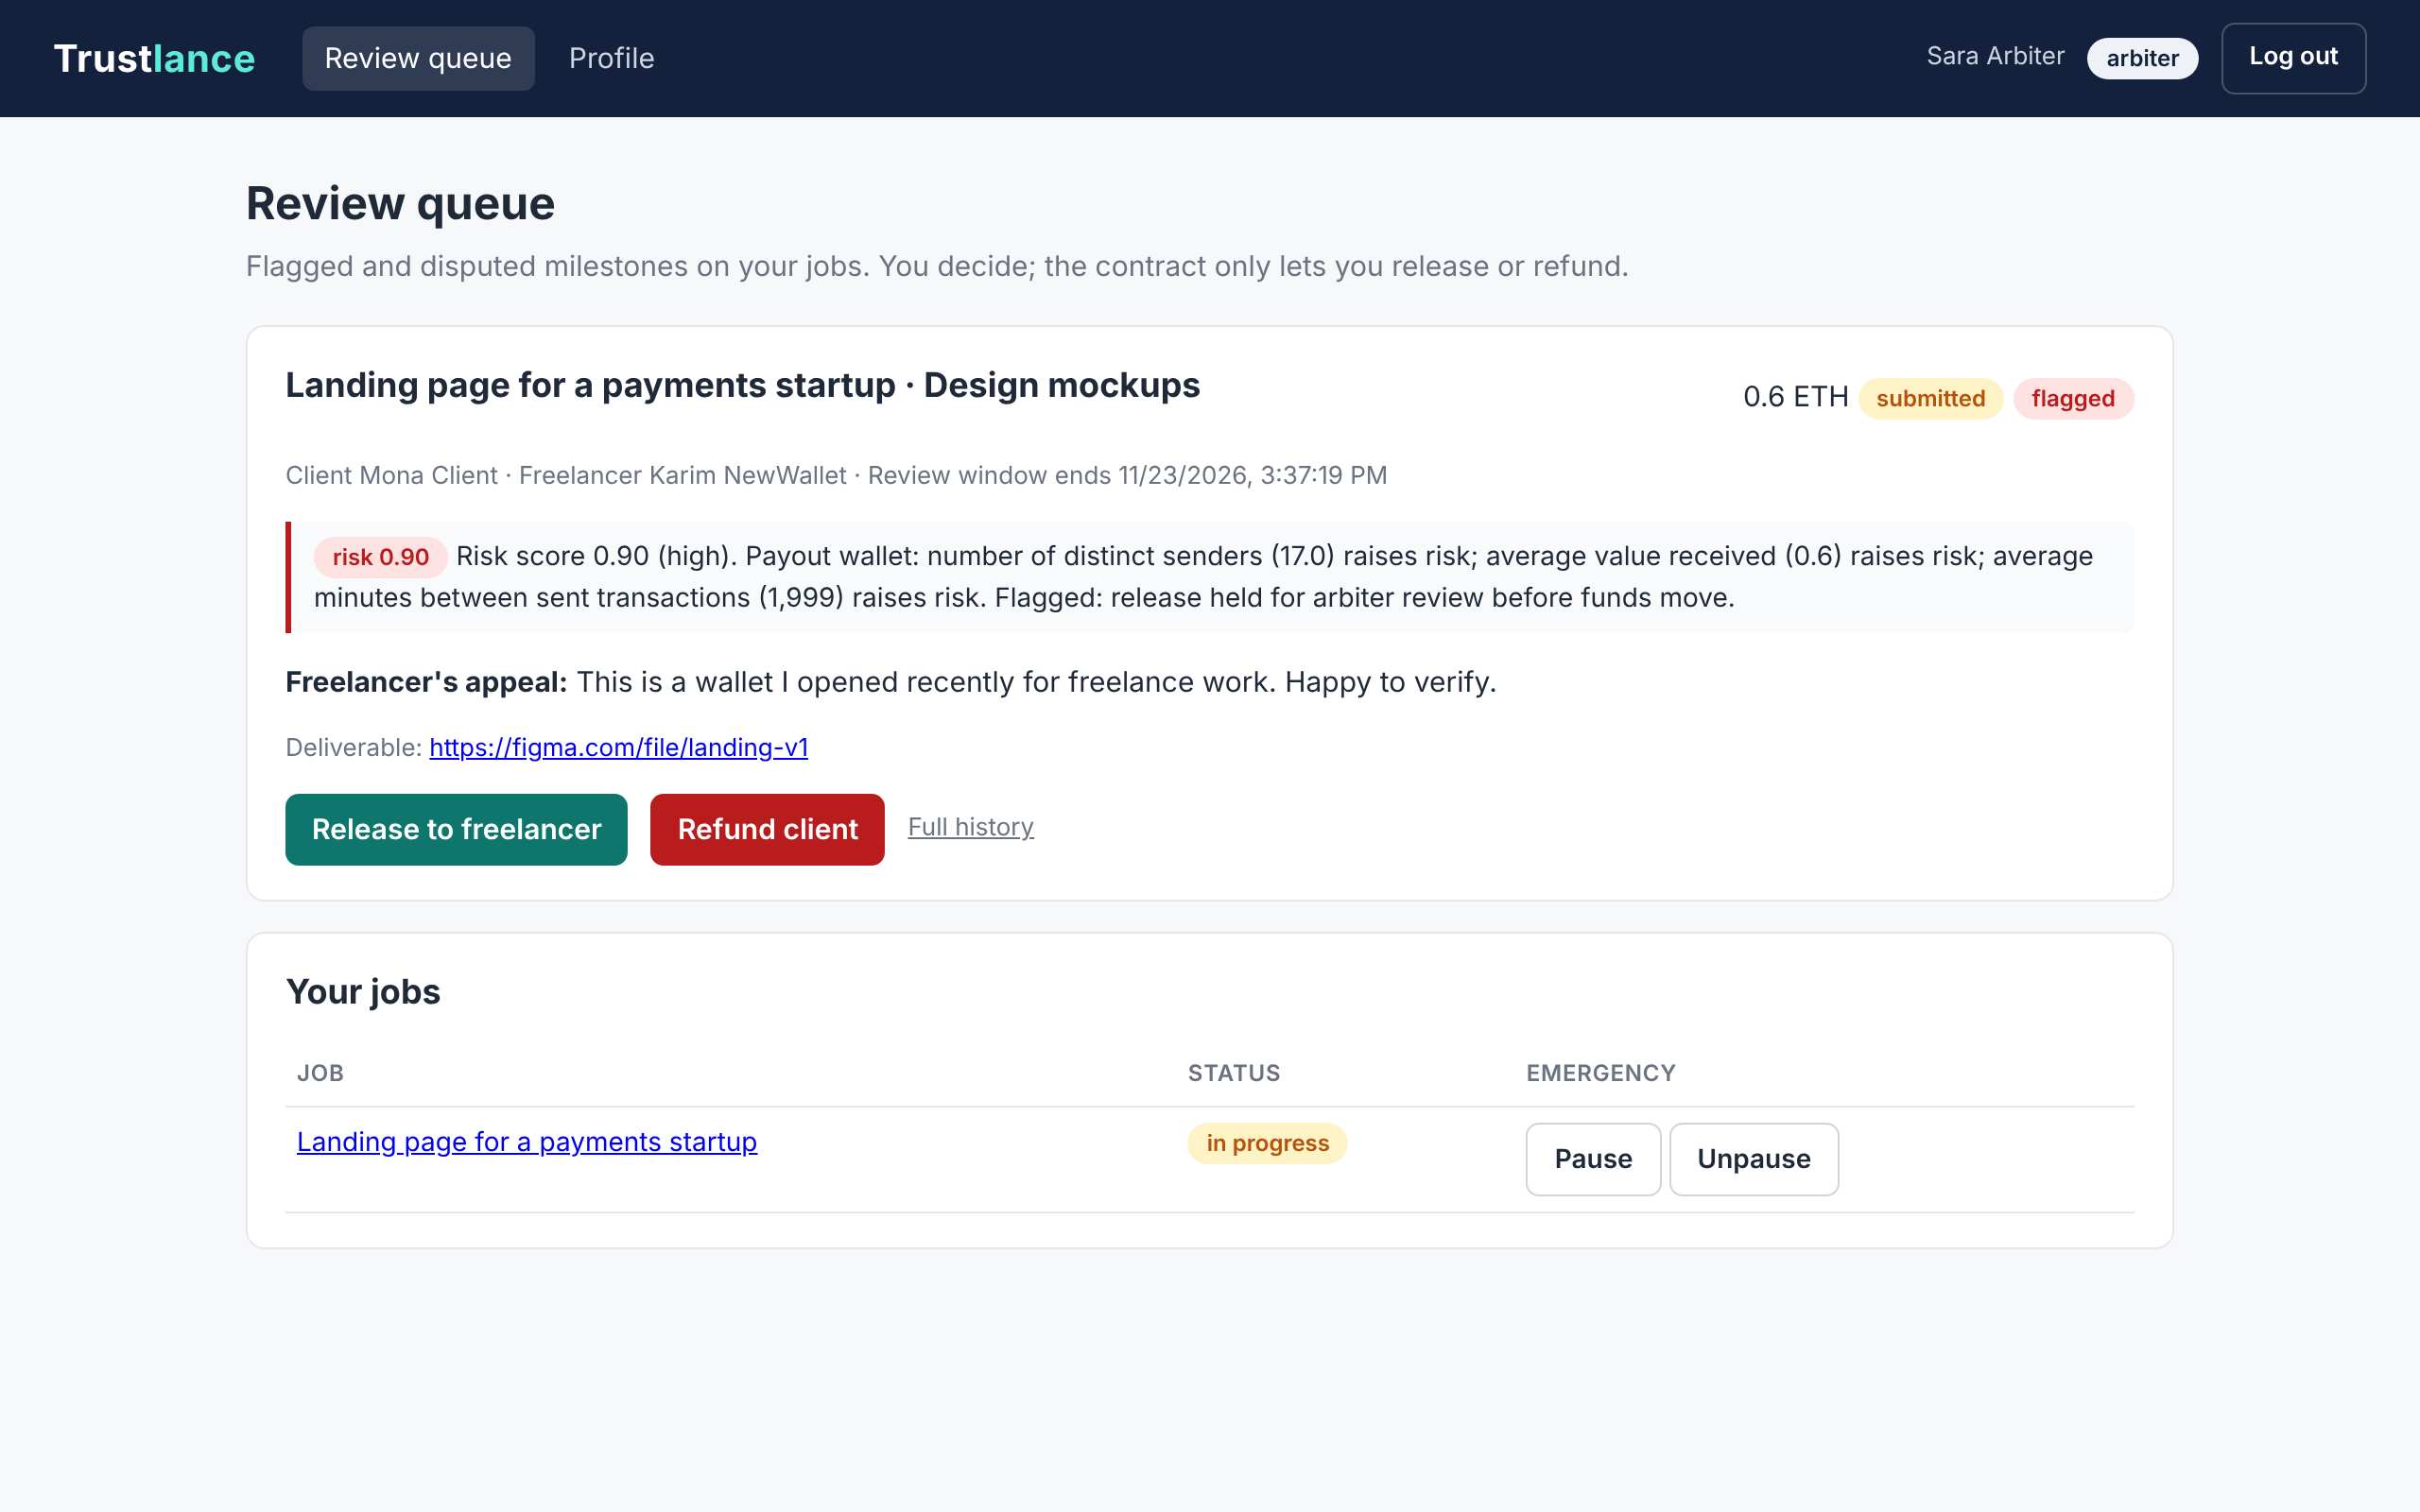
\includegraphics[width=0.92\textwidth]{figures/ui_arbiter_queue.png}
\caption{Arbiter's review queue with the score, the reason, the freelancer's appeal and the two possible decisions.}
\label{fig:ui-arbiter}
\end{figure}

\section{Testing}
There are 48 automated tests and all of them pass from a fresh copy of the repository.

\begin{table}[htbp]
\centering
\small
\begin{tabularx}{\textwidth}{>{\raggedright\arraybackslash}p{3.4cm}>{\centering\arraybackslash}p{1.2cm}L}
\hline
\textbf{Suite} & \textbf{Tests} & \textbf{What it covers} \\ \hline
Contract & 25 & Payment flow, risk hold, 7-day window, appeal, pause, roles, reentrancy attack \\
API & 11 & Accounts, roles, proposals, escrow deployment, low-risk release, high-risk hold with appeal and arbiter release, dispute and refund, pause \\
Python & 12 & Model quality on real data, bands and actions, audit-log tamper detection \\ \hline
\end{tabularx}
\caption{Automated tests.}
\label{tab:tests}
\end{table}

\section{How to run it}
The system needs Node.js 18 or later and Python 3. On Windows, in PowerShell:

\noindent\begin{minipage}{\linewidth}
\begin{lstlisting}
git clone https://github.com/alikhairyy/trustlance-poc
cd trustlance-poc
npm install
python -m venv .venv
.\.venv\Scripts\python.exe -m pip install -r risk-engine\requirements.txt
.\.venv\Scripts\python.exe risk-engine\fetch_real_data.py
npm run dev
\end{lstlisting}
\end{minipage}

Then open \texttt{http://localhost:3000}. All demo accounts use the password \texttt{demo1234}:
\begin{itemize}
\item \texttt{client@demo.com}, the client who owns a sample job;
\item \texttt{freelancer@demo.com}, a freelancer with a low-risk wallet;
\item \texttt{risky@demo.com}, a freelancer whose wallet the dataset labels as fraud;
\item \texttt{arbiter@demo.com}, the arbiter.
\end{itemize}
\texttt{npm test} runs the contract and API tests.

\section{Next steps}
\begin{enumerate}
\item Replace the server-held test wallets with MetaMask signing (FR18).
\item Deploy to a public test network and read real wallet history from a block explorer (FR9).
\item Deliver notifications and build ratings (FR16, FR17).
\item Run the survey and a small pilot, add freelancer-history signals to the model and tune the thresholds (FR19).
\end{enumerate}
